\documentclass[12pt]{report}
\usepackage[margin=1in]{geometry}
\usepackage{setspace} % for single/doublespacing commands
\usepackage{graphicx} % including graphics
\usepackage{sectsty} % sexy section headings
\usepackage{pdfpages} % including multipage pdfs
\usepackage[export]{adjustbox} % for graphic frames and center
\usepackage{siunitx}
\usepackage[numbered]{matlab-prettifier} % including matlab w/ syntax highlighting
\usepackage[T1]{fontenc} % prettier matlab font
\usepackage{xfrac} % more legible inline fractions (\sfrac)
\usepackage{lmodern} % font package for above
\usepackage{multicol} % multiple columns
\usepackage[justification=centering]{caption} % figure captions (force centering)
\usepackage{amsmath} % more math symbols and shit
\usepackage{enumitem} % add arguments for enumerate to change style
\usepackage[list=true]{subcaption} % subfigures with list of figure support
\usepackage{multirow}
\usepackage{mathtools}
\usepackage{booktabs}
\usepackage{color}
\usepackage{ulem}
\usepackage{blindtext}
\usepackage[numbers]{natbib}
\usepackage{contour}
\usepackage{tabularx}
\usepackage{circuitikz} % drawing fancy shit
\usepackage{cancel} % arrow and cross math cancel symbol
\usepackage{lineno}
\usepackage{framed}
\usepackage{amssymb} % special math symbols
\usepackage{listings}
\usepackage{array}
\usepackage{BOONDOX-cal} % fancy mathtype script
\usepackage{fancyhdr}
\usepackage{flowchart}
\usepackage{color, colortbl}
\usepackage{tocloft}
\usepackage{url}
\usepackage{etoolbox}
% \usepackage{hyperref}

\setlength{\parskip}{\baselineskip}%
\setlength{\parindent}{0pt}%
\setcounter{secnumdepth}{5}
\renewcommand{\bibname}{References}
\sisetup{output-exponent-marker=\ensuremath{\mathrm{e}}}
\newcommand{\PreserveBackslash}[1]{\let\temp=\\#1\let\\=\temp}
\newcolumntype{C}[1]{>{\PreserveBackslash\centering}p{#1}}
\newcolumntype{R}[1]{>{\PreserveBackslash\raggedleft}p{#1}}
\newcolumntype{L}[1]{>{\PreserveBackslash\raggedright}p{#1}}
\lstMakeShortInline[style=Matlab-editor]| % matlab inline escape character
\graphicspath{{images/}}
\renewcommand\thesection{\arabic{section}}
\renewcommand\labelitemi{---}
\lstset{numberstyle=\ttfamily\small\color{gray}}
\renewcommand\linenumberfont{\ttfamily\small\color{gray}}
\setlength\linenumbersep{6mm}
% \hbadness=99999  % or any number >=10000
\apptocmd{\sloppy}{\hbadness 10000\relax}{}{}
\usetikzlibrary{arrows,calc,patterns,angles,quotes}
% \usetikzlibrary{shapes.geometric}
% \usetikzlibrary{decorations.pathmorphing,decorations.pathreplacing} % for snakes!
% \usetikzlibrary{positioning, circuits.logic.US}
\setlength{\cftbeforetoctitleskip}{-2em}
\newcommand{\Lag}{\mathcal{L}} % lagrangian L

\apptocmd{\sloppy}{\hbadness 10000\relax}{}{}
\setlength{\cftbeforetoctitleskip}{-2em}
\allsectionsfont{\raggedright}
\setlist[enumerate]{wide=0pt, widest=99,
                    leftmargin=\parindent,topsep=0pt,partopsep=0pt,
                    label=\thesubsubsection.\alph*,font=\itshape}
\begin{document}
\normalem
\begin{titlepage}
\flushleft
\doublespacing
\Large
\textsc{Test Document} \\
\normalsize
Trey Dufrene, Zack Johnson, David Orcutt, Alan Wallingford, Ryan Warner
\vfill
\center
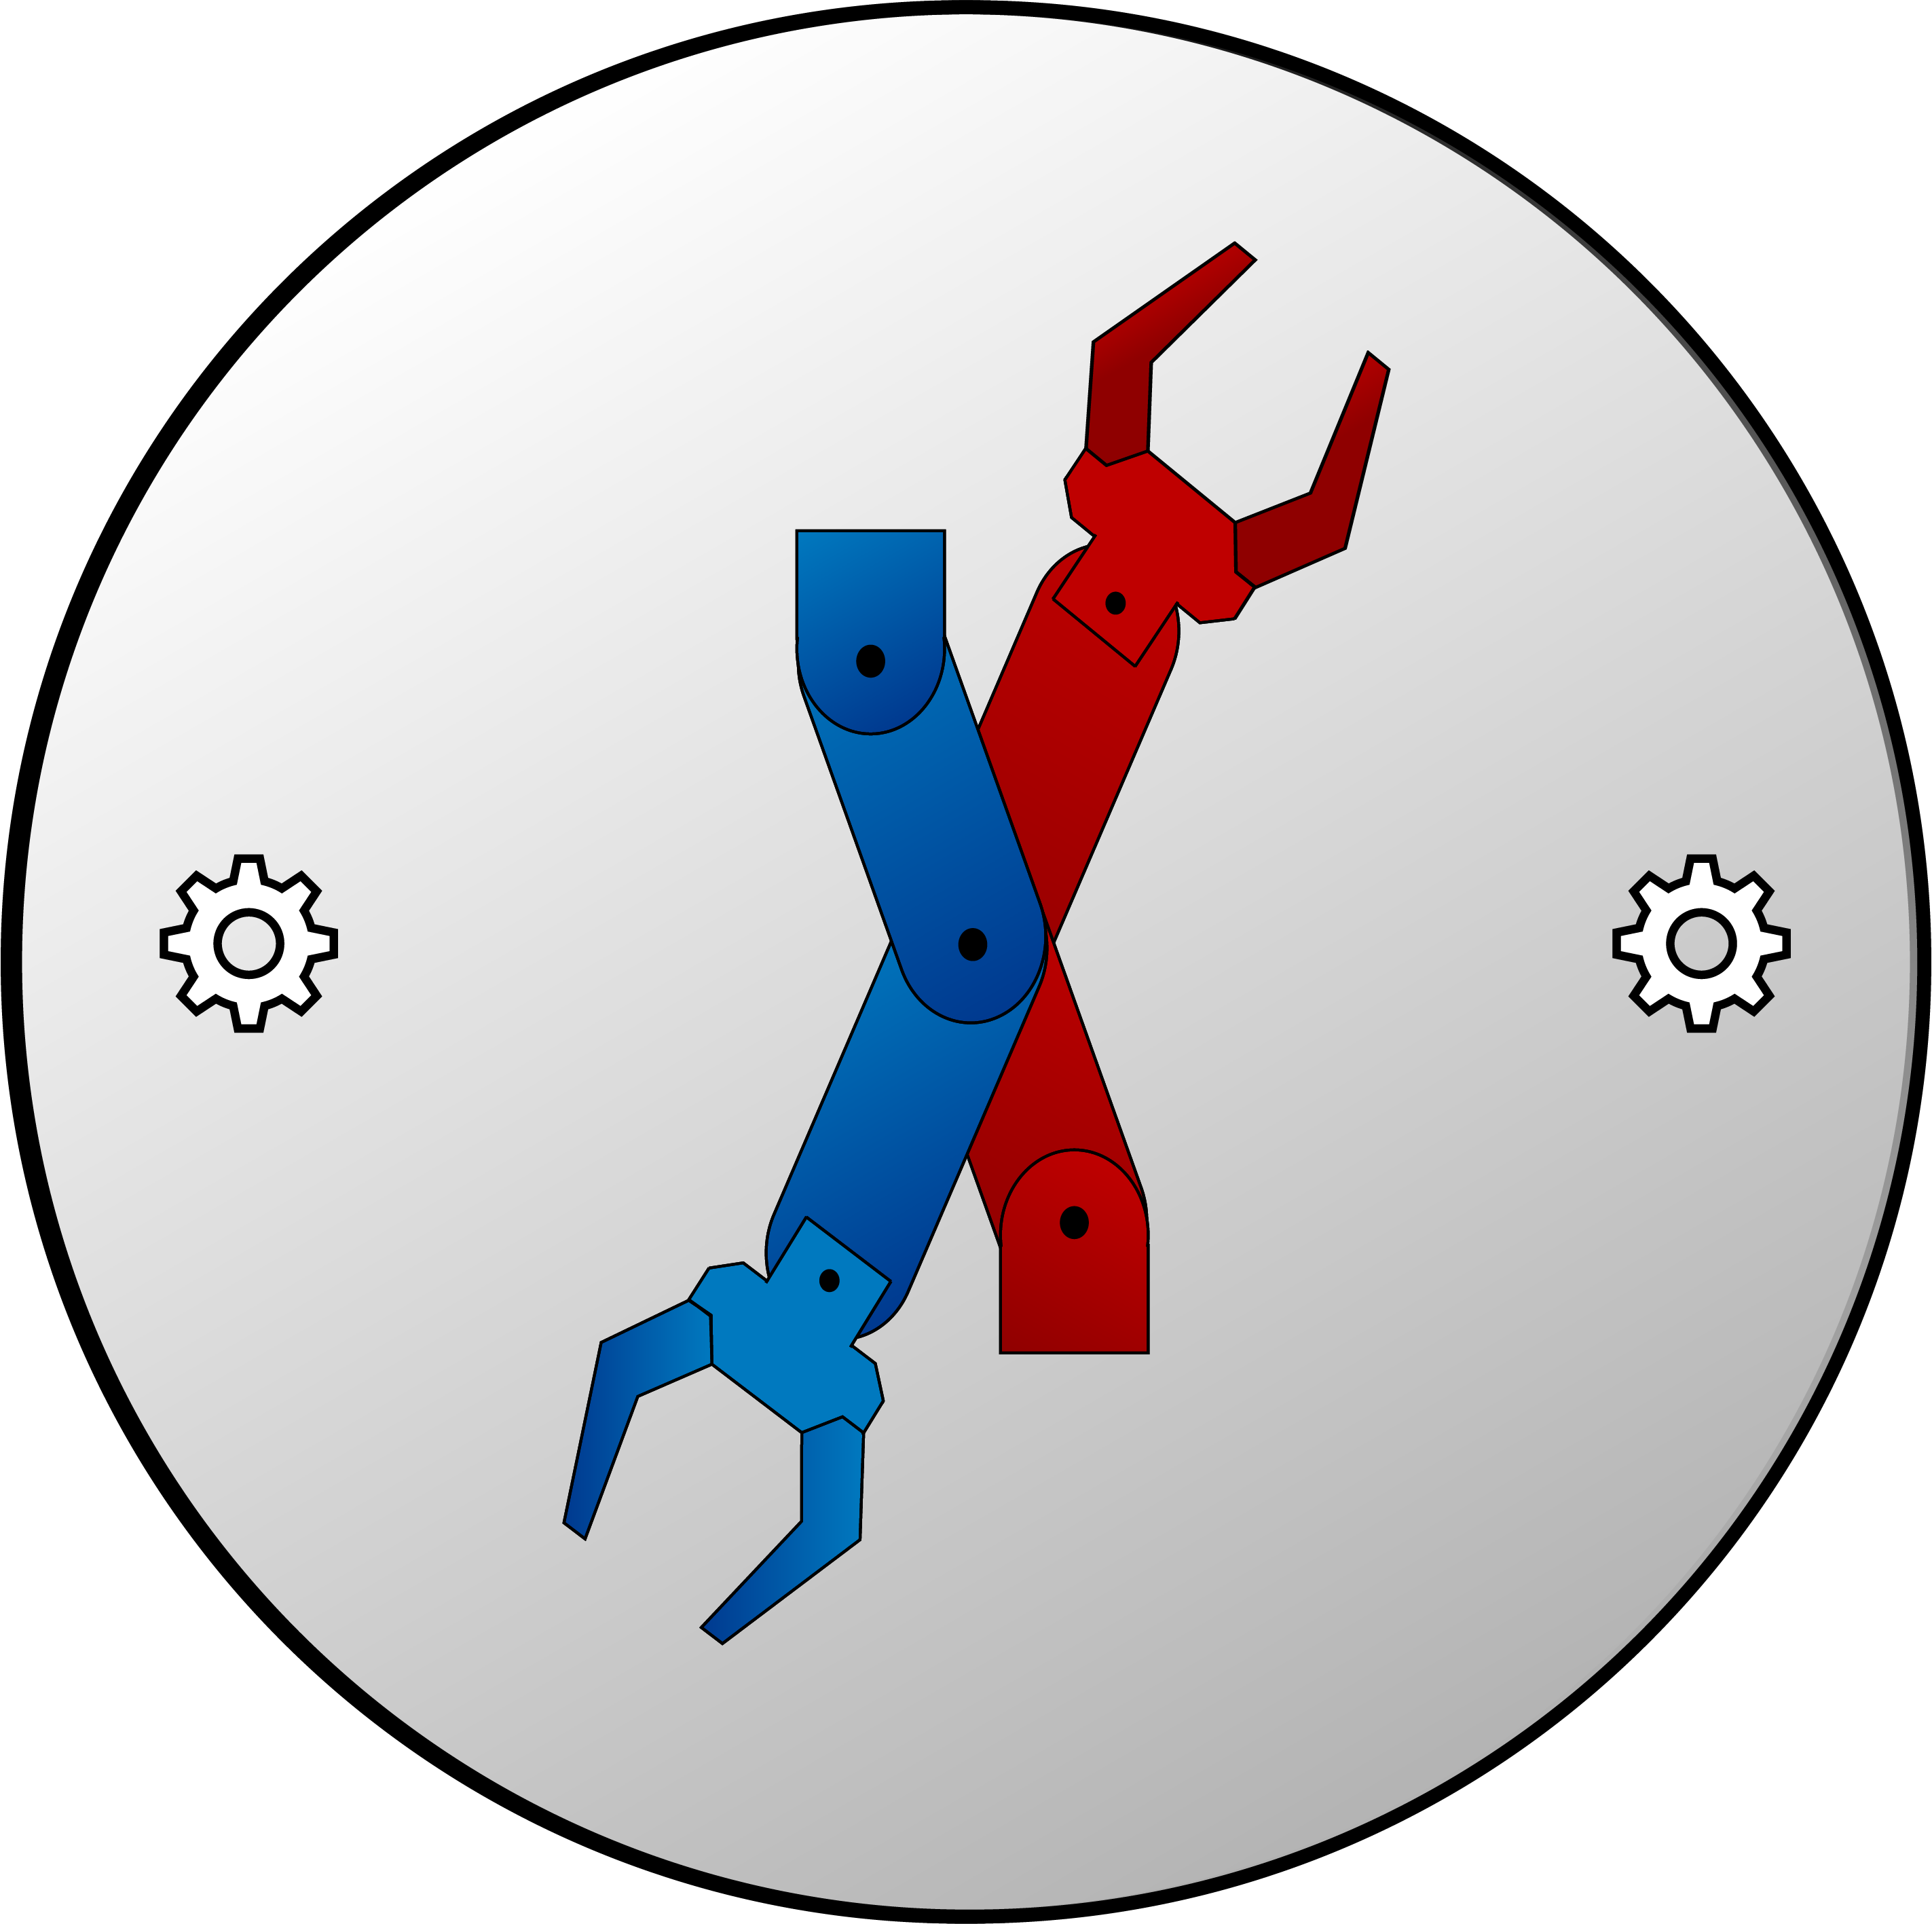
\includegraphics[width=.45\textwidth]{logo}
\vfill
\flushleft
ME 407 \\
Preliminary Design of Robotic Systems \\
Embry-Riddle Aeronautical University \\
\vspace{2ex}
\begin{minipage}[c]{.5\textwidth}
\flushleft

\includegraphics[width=.95\textwidth]{erau}
\end{minipage}%
\begin{minipage}[c]{.5\textwidth}
\flushright

\includegraphics[width=.8\textwidth]{text}
\end{minipage}
\end{titlepage}

\pagenumbering{roman}
% \begin{abstract}
  % Wordy words
% \end{abstract}
{\tableofcontents\let\clearpage\relax\listoffigures\let\clearpage\relax\listoftables}
\clearpage
\newpage

% \section*{List Of Acronyms and Abbreviations}

% \begin{tabular}{rl}
%   $G$~:&Center of gravity of the bar \\
%   $\ell_0$~:& Spring unstretched length  \\
%   $\delta$~:& Spring deflection \\
%   $k$~:& Spring constant \\
%   $h_{b}$~:& Distance to bar ($G$) from datum \\
%   $F_s$~:& Force onto bar due to spring\\
%   $A_{n}$~:& Pin reaction in $\theta$ direction\\
%   $A_{t}$~:& Pin reaction in tangential direction \\
%   $\vec{v}_G$~:& Velocity of bar center of gravity\\
%   $\ddot{\theta}$~:& Angular velocity of spring \\
%   $\ddot{\phi}$~:& Angular velocity of bar\\
%   $\ddot{\ell}_s$~:& Radial acceleration of spring \\
% \end{tabular}
% \normalsize
% \flushleft
% \singlespacing
% \newpage

\pagenumbering{arabic}
\section{Introduction}
\section{Requirements}
\section{Conceptual Design}
\section{Specifications}
\newpage
\section{Preliminary Design}
\subsection{CAD}
\subsection{Forward Kinematics}
\subsection{Velocity Kinematics}
\subsection{Inverse Kinematics}
\subsection{Equations of Motion}
\subsection{Open-Loop Simulation}
\subsection{Control System}
\subsection{Closed-Loop Simulation}
\subsection{ANSYS}
\subsection{Electrical Schematic}
\subsection{Software Flowchart}
\subsection{Project Status and Future}
\subsection{Parts List}

\newpage


\begin{figure}[htp]
  \centering
  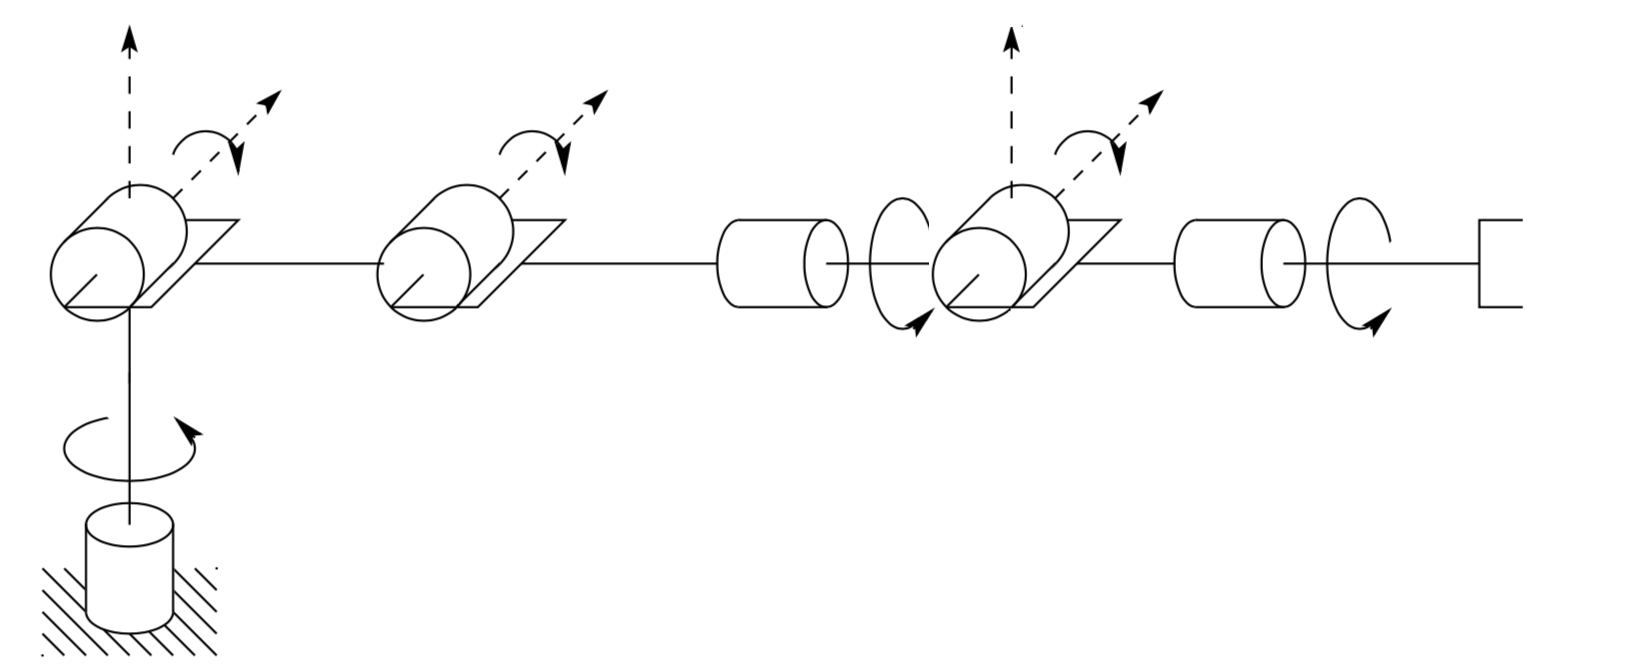
\includegraphics[width=.9\textwidth]{zero}
  \caption{Coordinate Systems}
  \label{fig:coords}
\end{figure}


Where \(\ell_1 = 22.08\)cm, \(\ell_2 = 25\)cm, \(\ell_3 = 20\)cm, \(\ell_4 = 8\)cm, \(\ell_6 = 5.25\)cm, and \(d = 1\)cm.


\[
A_1 = rotz(\theta_1) ~ transz(\ell_1) ~ rotx(\sfrac{\pi}{2})
\]
\vspace{.25ex}
\[
A_1 =
\begin{bmatrix}
  \cos(\theta_1) & 0 & \sin(\theta_1) & 0 \\
  \sin(\theta_1) & 0 & -\cos(\theta_1) & 0 \\
  0 & 1 & 0 & 22.08 \\
  0 & 0 & 0 & 1 \\
\end{bmatrix}
\]
\vspace{.25ex}
\[
A_2 = rotz(\theta_2) ~ transz(-d) ~ transx(\ell_2)
\]
\vspace{.25ex}
\[
A_2 =
\begin{bmatrix}
  \cos(\theta_2) & -\sin(\theta_2) & 0 & 25\cos(\theta_2) \\
  \sin(\theta_2) & \cos(\theta_2) & 0 & 25\sin(\theta_2) \\
  0 & 0 & 1 & -1 \\
  0 & 0 & 0 & 1 \\
\end{bmatrix}
\]
\vspace{.25ex}
\[
A_3 = rotz(\theta_3 + \sfrac{\pi}{2}) ~ rotx(\sfrac{\pi}{2})
\]
\vspace{.25ex}
\[
A_3 =
\begin{bmatrix}
  \cos(\theta_3 +  \sfrac{\pi}{2}) & 0 & \sin(\theta_3 +  \sfrac{\pi}{2}) & 0 \\
  \sin(\theta_3 +  \sfrac{\pi}{2}) & 0 & -\cos(\theta_3 +  \sfrac{\pi}{2}) & 0 \\
  0 & 1 & 0 & 0 \\
  0 & 0 & 0 & 1 \\
\end{bmatrix}
\]
\vspace{.25ex}
\[
A_4 = rotz(\theta_4) ~ transz(\ell_3 + \ell_4) ~ rotx(-\sfrac{\pi}{2})
\]
\vspace{.25ex}
\[
A_4 =
\begin{bmatrix}
  \cos(\theta_4) & 0 & -\sin(\theta_4) & 0 \\
  \sin(\theta_4) & 0 & \cos(\theta_4) & 0 \\
  0 & -1 & 0 & 28 \\
  0 & 0 & 0 & 1 \\
\end{bmatrix}
\]
\vspace{.25ex}
\[
A_5 = rotz(\theta_5) ~ rotx(\sfrac{\pi}{2})
\]
\vspace{.25ex}
\[
A_5 =
\begin{bmatrix}
  \cos(\theta_5) & 0 & \sin(\theta_5) & 0 \\
  \sin(\theta_5) & 0 & -\cos(\theta_5) & 0 \\
  0 & 1 & 0 & 0 \\
  0 & 0 & 0 & 1 \\
\end{bmatrix}
\]
\vspace{.25ex}
\[
A_6 = rotz(\theta_6) ~ transz(\ell_6)
\]
\vspace{.5ex}
\[
A_6 =
\begin{bmatrix}
  \cos(\theta_6) & 0 & -\sin(\theta_6) & 0 \\
  \sin(\theta_6) & 0 & \cos(\theta_6) & 0 \\
  0 & 0 & 1 & 5.25 \\
  0 & 0 & 0 & 1 \\
\end{bmatrix}
\]

\newpage

\section{Motor Dynamics}
Given robot dynamics described by \(H(\gamma)\ddot{\gamma} + n(\gamma,\dot{\gamma}) = \tau\), the torque, $\tau$, provided by the servo motors is necessary to solve the closed loop dynamics of the system. Assuming the servo is driven by a D.C. motor with proportional derivative control,
\begin{equation}
  \tau_a = Ki_a = J_a\ddot{\theta}_a + b_a\dot{\theta}_a + \tau_L
  \label{eq:motor}
\end{equation}
Where $\tau_a$ is the actuator torque, $K$ is the back-EMF constant, $i_a$ is the motor current, $J_a$ is the armature inertia, $\theta_a,~\dot{\theta}_a,\ddot{\theta}_a$ is the motor position and it's first and second time derivatives, respectively, $b_a$ is the viscous friction coefficient, and $\tau_L$ is the torque available for the actuator to do work. The basic equation for a motor is known to be:
\begin{equation}
  V_a = i_aR_a + K\dot{\theta}_a
  \label{eq:va}
\end{equation}
Where $V_a$ is the voltage applied to the actuator and $R_a$ is the armature resistance. Given a gearbox with $\sfrac{\text{in}}{\text{out}}$ ratio $N$ and efficiency $\eta$,
\begin{center}
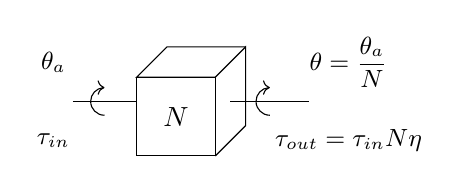
\begin{tikzpicture}
\pgfmathsetmacro{\cubex}{1}
\pgfmathsetmacro{\cubey}{1}
\pgfmathsetmacro{\cubez}{1}
\draw (0,0,0) -- ++(-\cubex,0,0) -- ++(0,-\cubey,0) -- ++(\cubex,0,0) -- cycle;
\draw (0,0,0) -- ++(0,0,-\cubez) -- ++(0,-\cubey,0) -- ++(0,0,\cubez);
\draw (0,0,0) -- ++(-\cubex,0,0) -- ++(0,0,-\cubez) -- ++(\cubex,0,0);
\draw (-2,-.5,-.5) -- ++(.8,0,0) node(a)[midway,above]{} node(b)[midway]{} node(c)[midway,below]{};
\pic [draw,angle radius=5,<-] {angle = a--b--c};
\node at (-2.25,0,-.5) {\small $\theta_a$};
\node at (-2.25,-1,-.5) {\small $\tau_{in}$};
\draw (0,-.5,-.5) -- ++(1,0,0);
\draw (0,-.5,-.5) -- ++(1,0,0) node(a1)[midway,above]{} node(b1)[midway]{} node(c1)[midway,below]{};
\pic [draw,angle radius=5,<-] {angle = a1--b1--c1};
\node at (1.5,0,-.5) {\small $\theta=\dfrac{\theta_a}{N}$};
\node at (1.5,-1,-.5) {\small $\tau_{out}=\tau_{in}N\eta$};
\node at (-.5,-.5,0) {$N$};
\end{tikzpicture}
\end{center}

The motor equation (\ref{eq:motor}) can be expressed in the output coordinates:
\[
Ki_a = J_aN\ddot{\theta} + b_aN\dot{\theta} + \frac{\tau}{N\eta}
\]
Substituing into equation (\ref{eq:va}) and solving for $i_a$:
\[
  i_a = \frac{J_aN}{K}\ddot{\theta} + b_aN\dot{\theta} + \frac{\tau}{N\eta}
\]
\begin{equation}
  V_a = \frac{R_aJ_aN}{K}\ddot{\theta} + \frac{R_ab_aN}{K}\dot{\theta} + \frac{R_a}{KN\eta}\tau + KN\dot{\theta}
  \label{eq:newva}
\end{equation}
Assuming P.D. control, \(V_a = K_p(\theta-\theta_d) + K_d\dot{\theta}\), where $\theta_d$ is the desired orientation of the actuator, the following solution is found by setting the P.D. solution equal to (\ref{eq:newva}). After collecting like terms:

\begin{equation}
  \frac{R_aJ_aN}{K}\ddot{\theta} + \left( \frac{R_aJ_aN}{K} - K_d + KN \right)\dot{\theta} - K_p\theta = -K_p\theta_d - \frac{R_a}{KN\eta}\tau
  \label{eq:end1}
\end{equation}
\newpage
The following parameters of the system can be obtained by applying a step input to the system with $\tau=0$ and measuring the characteristics of it's response. Denoting $\zeta$ as the damping ratio and $\omega_n$ as the natural frequency of the system,
\[
  \text{\% Overshoot} = \left( \frac{\theta_{max} - \theta_{ss}}{\theta_{ss}} \right) \times 100~,\quad \zeta = \frac{-\ln(\sfrac{\%\text{OS}}{100})}{\sqrt{\pi^2 + \ln^2(\sfrac{\%\text{OS}}{100})}}~,\quad \omega_n = \frac{\pi}{T_p\sqrt{1-\zeta^2}}
\]

Given $\theta_{max},~\theta_{ss},$ and $T_p$ as measured parameters of the system's max output, steady state, and time to peak, respectively.

Refactoring equation (\ref{eq:end1}) and equating with the general solution for a second order system given by $\ddot{\theta} + 2\zeta\omega_n\dot{\theta} + \omega_n^2\theta = \omega_n^2\theta_d$,
\begin{equation}
  2\zeta\omega_n = \frac{b_a}{J_a} - \frac{KK_d}{R_aJ_aN} + \frac{K^2}{R_aJ_a}~,\quad
  \omega_n^2 = \frac{-KK_p}{R_aJ_aN}
\end{equation}
Performing a similar experiment as previously described, except with a known inertial load $\tau = J_m\ddot{\theta}$, the following parameters can be found:
\begin{equation}
  \alpha_m \equiv 2\zeta\omega_n = \frac{R_ab_aN^2\eta-KK_dN\eta+K^2N^2\eta}{R_aJ_aN^2\eta+R_aJ_m}~,\quad
  \beta_m \equiv \omega_n =-\frac{KK_pN\eta}{R_aJ_aN^2\eta+R_aJ_m}
\end{equation}

\begin{equation}
\begin{bmatrix}
  1 & -(\alpha_1J_1+\beta_1J_1) \\
  1 & -(\alpha_2J_2+\beta_2J_2) \\
  \vdots & \vdots
\end{bmatrix}
\begin{bmatrix}
  \dfrac{R_ab_aN^2\eta-KK_dN\eta+K^2N^2\eta-KK_pN\eta}{R_aJ_aN^2\eta} \\
  ~\\
  \dfrac{1}{J_aN^2\eta}
\end{bmatrix}
=
\begin{bmatrix}
  \alpha_1+\beta_1 \\
  \alpha_2+\beta_2 \\
  \vdots
\end{bmatrix}
\label{eq:soe}
\end{equation}
Finally, with multiple datasets (varying inertial loads, $J_m$) the coefficients of the second order system equation can be found using the least squares solution of (\ref{eq:soe}).





% \begin{enumerate}[label=\alph*.]
%   \item Description for callout a
%   \item Description for callout b
% \end{enumerate}

% Example citations:
% \cite{DBLP:journals/corr/JohnsonAL16}
% \cite{DBLP:journals/corr/abs-1803-09820}
% \cite{DBLP:journals/corr/RonnebergerFB15}

% \newpage
% \bibliographystyle{plain}
% \bibliography{JohnsonAL16,abs-1803-09820,RonnebergerFB15}

\newpage
\section*{Acknowledgements \& Attributions}
We would like to acknowledge the following people for their contibutions to creating this report?
\begin{itemize}
  \item Dr. Isenberg
\end{itemize}

\newpage
\appendix
\renewcommand\thesection{\Roman{section}}
\renewcommand\thesubsection{\roman{subsection}}
\section{Appendix}\label{sec:app}
\subsection{Drawings}
\subsection{Salient Code}
% Code listing
%\begin{lstlisting}[frame=lines,style=Matlab-editor,basicstyle = \mlttfamily, caption=Example Code
% Code Here
%\end{lstlisting}
% \includepdf[landscape,pages=-]{pdfname}

\end{document}
